\documentclass{article}
\usepackage[utf8]{inputenc}

\title{Visualization of Prim's Algorithm}
\author{Joel P. Abraham }
\date{December 12, 2016}

\usepackage{graphicx}
\usepackage{caption}
\usepackage{subcaption}


\begin{document}

\maketitle

\section{Introduction}
Throughout this semester, I’ve researched my topic of algorithm design and analysis extensively, and have gained significant insight into the process by which a problem is identified and an algorithmic solution is produced. I’ve learned about the various design paradigms that are central in the construction of algorithms as well as the various methods by which algorithms can be characterized, such as time and space complexity. Furthermore, I’ve learned about specific techniques of algorithm design that are crucial to successfully and conveniently designing an optimal algorithm. These findings have been very valuable, not only for developing solutions to computing problems but also for problem-solving in general, as my research has gone beyond merely explaining solutions to specific problems, and rather demonstrated how abstract problems should be approached. 

For my final product, synthesizing all the research I have conducted over the course of this semester, I designed a program to visualize Prim’s Algorithm, a greedy approach to finding the minimum spanning tree of a connected, edge-weighted, undirected graph. This is useful, not merely to demonstrate the knowledge I have gained throughout my research or to actually find minimum spanning trees, but also as an educational tool to help understand greedy algorithms in general, as my program displays each iteration of Prim’s Algorithm, coherently indicating how locally optimal choices sum together to yield a general solution.

\section{Summary of Findings}

My research has yielded many strategies for algorithm design, the most important of which is modeling problems intuitively; this can be immensely valuable, as it enables a deeper understanding of the problem, and can simplify a seemingly complex problem into a trivial one. Computer science problems are often obfuscated by generalizations (solving for n-cases) or academic jargon, such as the peak-finding problem, which states “Given array $A[0, 1…n-1], A[i]$ is a peak if it is not smaller than both of its neighbors $(A[i+1], A[i-1])$, find any peak.” This appears difficult, when in actuality the problem is simply asking for any local maximum value. When problems are modeled intuitively, the problems become less abstract and more concrete, and common sense can be often be applied to yield an efficient, obvious solution. An excellent example, which was included in a previous presentation of mine, is the Stable Marriage Problem, which states “Given two equally sized sets of n elements with an order of preferences for each element, find a stable matching, where a stable matching is defined to be a mapping from elements of one set to the other (i.e. construction of a bipartite graph) such that there does not exist a match that would be preferred by both elements.” This can be modeled intuitively using the example of marriage between men and women, where each man and woman ranks the elements of the opposite set by preference. From here, the solution is fairly simple, as exemplified by the demonstration which I conducted in class, since the students were able to solve the applied version of the problem with minimal assistance, and could then generalize to yield an solution to the general problem statement, arriving at the Gale-Shapley Algorithm. As such, modeling instances of the problem using real-world examples and later abstracting is a fundamental tactic that is invaluable when designing algorithms.

A second key strategy for problem-solving is the use of the various design paradigms which are well-established in computer science, namely brute force, recursion, divide and conquer, greedy, backtracking, branch and bound, and memoization. These approaches are useful for creating functional, efficient algorithms, as well as optimization. In my presentations, I’ve covered these design paradigms, and demonstrated many algorithms which are founded upon one or more of these central approaches. The greedy approach, in particular, is an excellent tool for approaching many problems; it relies on the observation that optimal solutions to local subproblems often constitute globally optimal solutions. Under this assumption, the problem can be reduced into its simpler subproblems, which often have trivial or relatively easy solutions. One prime example of this phenomenon is the interval scheduling problem, which states “Given n requests with each request i specifying a start time $s(i)$  and a finish time $f(i)$, find the maximum subset of requests such that all pairs of requests $i,j \in A$, i  ≠ j are compatible, where two requests i and j are compatible if the requested intervals do not overlap (i.e. $f(i) \leq s(j)$  or $f(j) \leq s(i)$).” Using the first strategy, this problem can be modeled through the scheduling of a resource, say a computer, in which case the problem is merely asking for the maximum set of non-overlapping intervals of time. Intuitively, to maximize the number of people who use the computer, we want the computer to be available as soon as possible, to allow for more time for others to use it, therefore we may consider the intervals that finish earliest. This is the crux of the greedy algorithm; the solution involves identifying the element with the earliest finish time, adding it to the solution set, and removing it along with all incompatible elements from the input set. Another application of  the greedy approach is its use to find minimum spanning trees in a graph, which I’ll address later, as it is the basis of my program. The greedy approach is particularly fascinating to me since it appears obvious in retrospect, almost like an oversimplification, but is rarely considered when approaching the problem. As such, the greedy approach and the other design paradigms are key techniques for designing algorithms, and different design paradigms are optimally configured for different types of tasks.

\section{Reflection of Experiences}

Given the above findings, my research can be described as relatively fruitful. Although I generally focused on a few problems, they were each representative of a different design paradigm, and I used them as springboards to explore certain approaches more thoroughly. My research process involved identifying an interesting, accessible computer science problem, exploring its algorithmic solutions, comparing their efficiencies, and classifying them by their general approach. This prompted a deeper investigation of each specific area, as I began to develop a more nuanced understanding of the process of algorithm design, learning which classes of algorithms are optimal for which types of problems. Occasionally, however, my progress would be impeded by a concept that I would fail to understand. In these situations, I would consult additional sources, or research background information so as to understand the topic contextually before attempting to further explore specifics. My sources include Wikipedia, for general information, TED Talks, computer science textbooks (Kleinberg and Tardos), university computer science resources, and online articles. With a combination of these sources, I was able to find all the information desired on my research topics. Furthermore, I communicated the information I learned through my research to the class, during my biweekly presentations; these presentations functioned as assessments of my own knowledge of the subject matter, and my instruction of the various research topics presented consummated my understanding while providing me with novel perspectives on these concepts.

Not only was this research successful, but it is also extremely useful for my future studies and career. Although I don’t plan to pursue a degree in computer science, I am interesting in continuing to learn computer science as I major in engineering—specifically chemical engineering. A solid understanding of algorithm design will be invaluable for me as I continue into college and study engineering, as there exists a significant overlap both conceptually and pragmatically. The concepts I’ve understood through my research will inevitably be important to engineering, but my research will also be beneficial, as it will enable me to effectively design and implement algorithms to solve problems computationally. Moreover, as I’ve stated earlier, the skills gained from my research can be generalized to apply to problem-solving as a whole, and are therefore useful in the construction of a conceptual framework for tackling the problems of every day life.

The research I conducted during the first semester on algorithm design was by no means comprehensive, and there is still a vast amount of unexplored information on this subject; while most of it remains inaccessible to me at this time, there is a plethora of easy to understand topic literature, which I plan to harness for future research. Although I have exhausted the low-hanging fruit, such as the various approaches to algorithm design, and have covered all of the of the fundamental design paradigms, areas in which I can delve further include amortized analysis, randomized algorithms, classification of problems and algorithms, and graph theory. Graph theory is a subset of discrete mathematics that is a fundamental structure in computer science, and graph traversal, transformation, connectivity, and analysis are all rich topics for algorithm design. I have already begun exploring this field, specifically looking at minimum spanning trees, which is the core of my final product; I will elaborate more on this in the following section.

\begin{figure}
\centering
\begin{subfigure}{.5\textwidth}
  \centering
  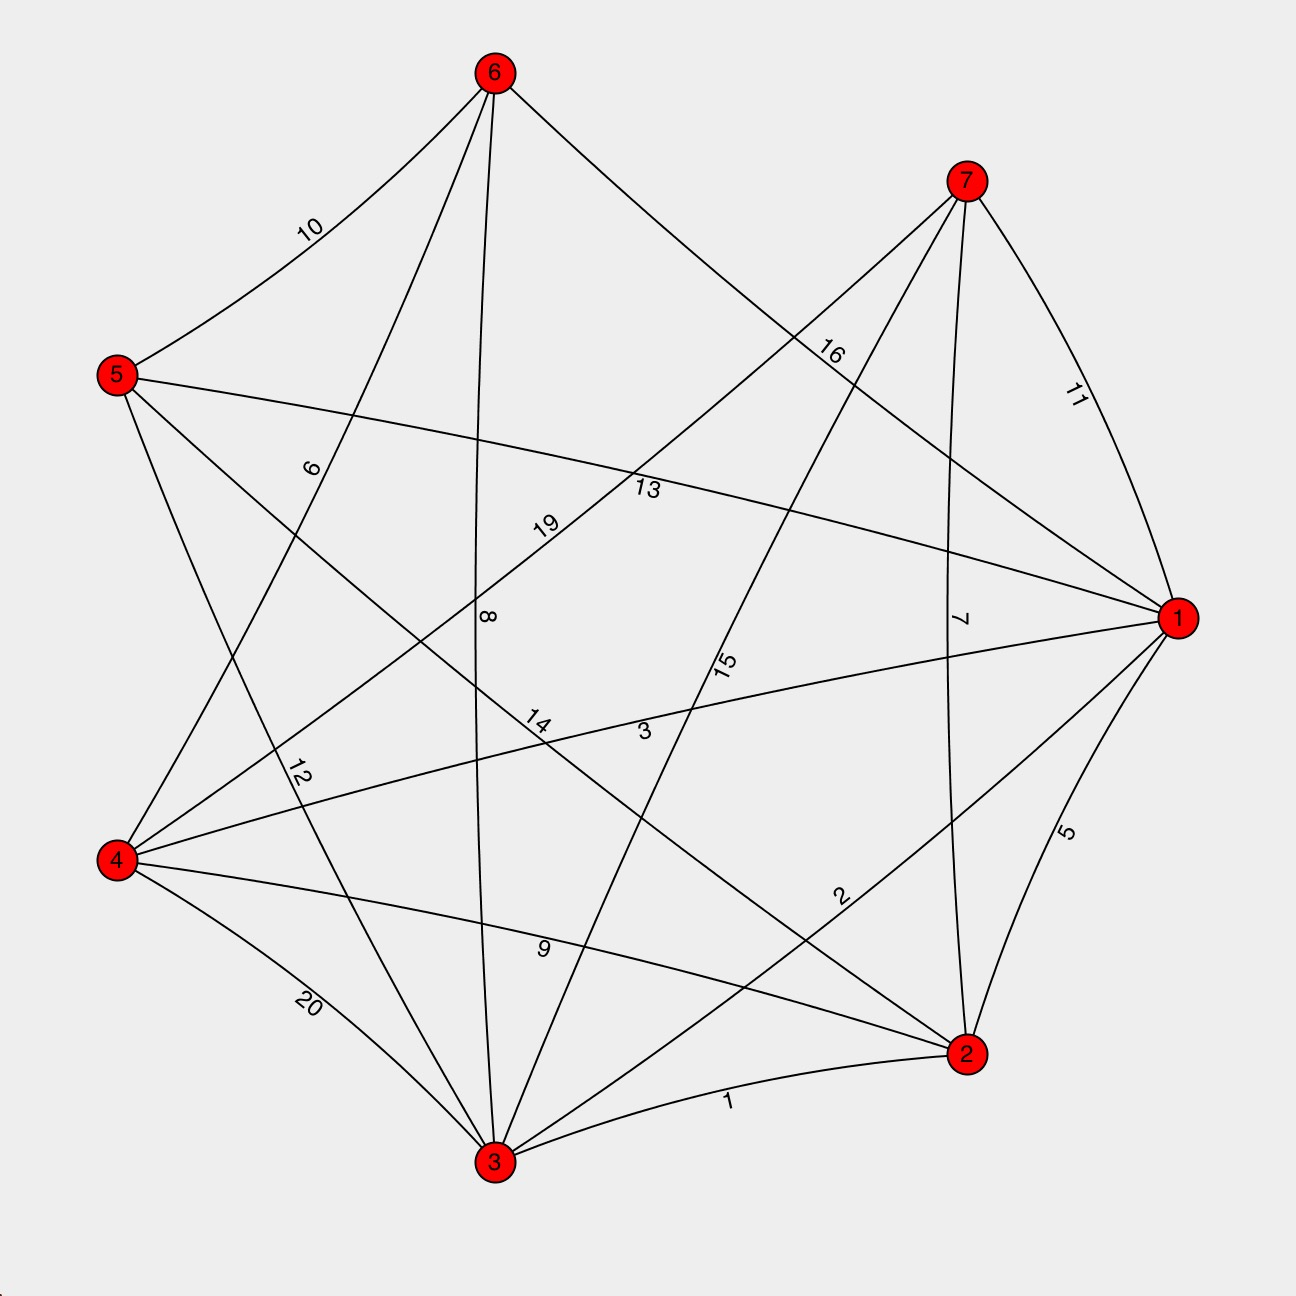
\includegraphics[width=.9\linewidth]{UDG.jpg}
  \caption{Undirected Dense Graph}
  \label{fig:sub1}
\end{subfigure}%
\begin{subfigure}{.5\textwidth}
  \centering
  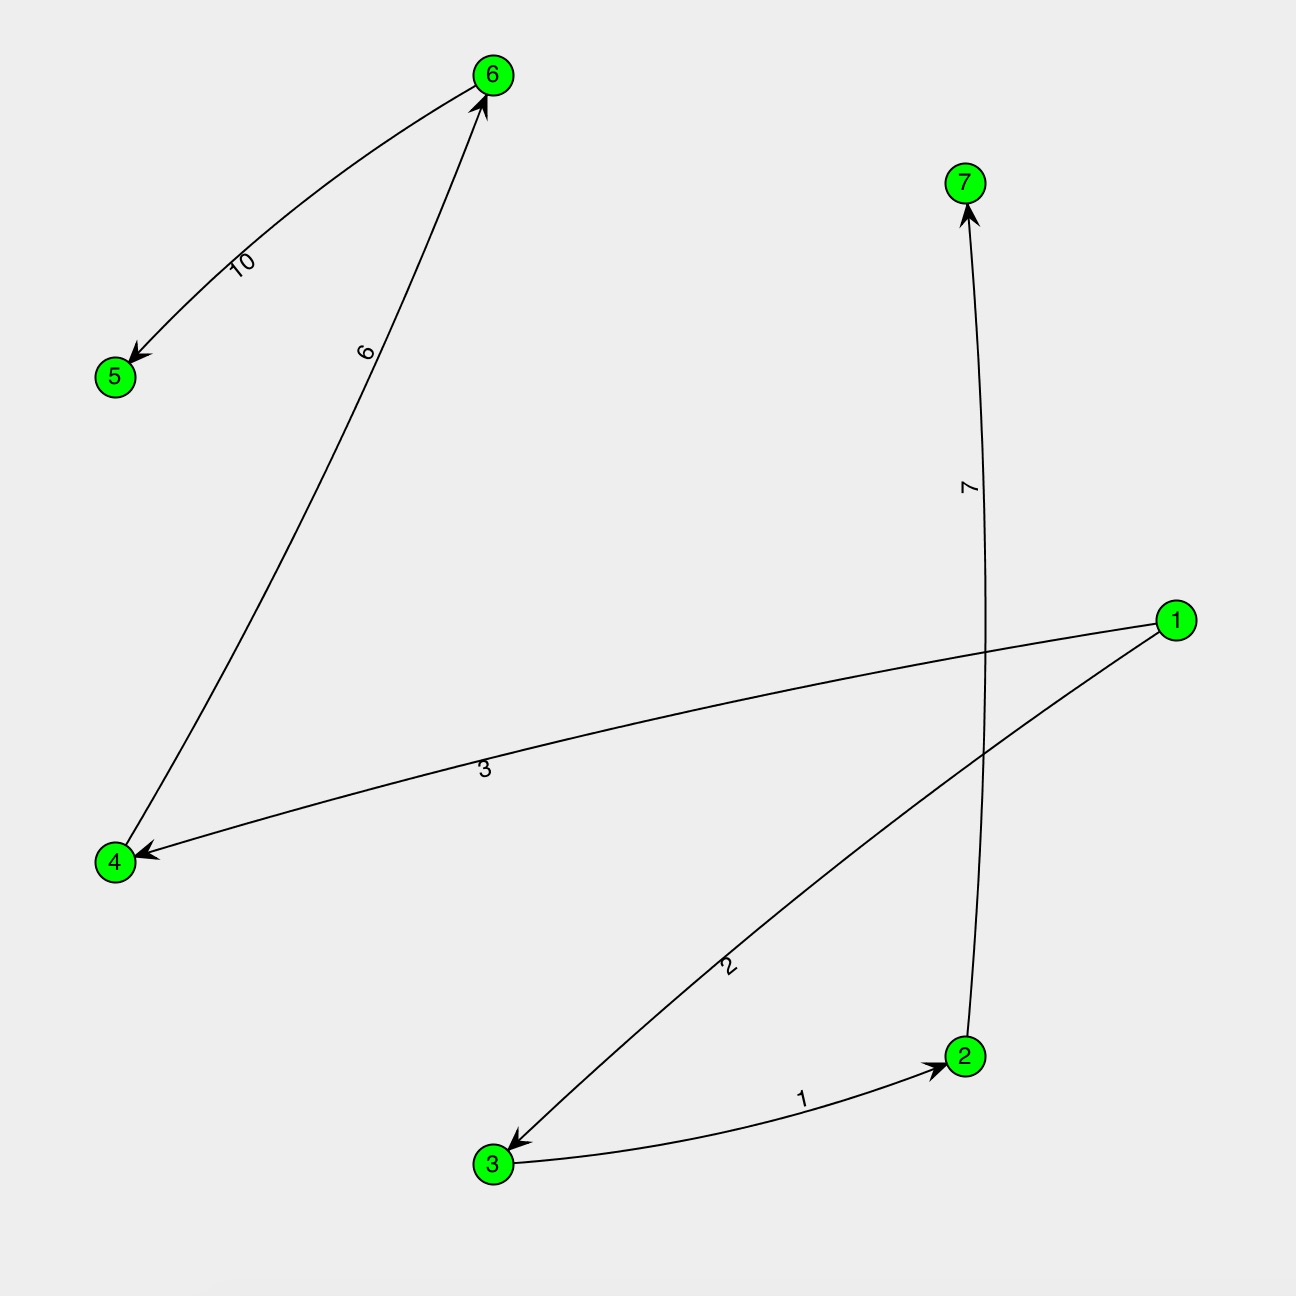
\includegraphics[width=.9\linewidth]{MST.jpg}
  \caption{Minimum Spanning Tree}
  \label{fig:sub2}
\end{subfigure}
\caption{Demonstration of Visualization with Arbitrarily Weighted Graph}
\label{fig:test}
\end{figure}


\section{Final Product: Visualization of Prim's Algorithm}

A fundamental problem in graph theory is finding the minimum spanning tree—the tree that connects all the vertices of a graph with minimally weighted edges to yield the minimum net cost—of a connected, edge-weighted, undirected graph (Fig. 1). Much work has gone into this problem, and the dominant solutions all utilize a greedy approach, exploiting the observation that given any vertex on the graph, the minimum spanning tree necessarily includes the minimally weighted edge incident to that vertex. This is easily understood: if we assume the converse to be true, that the minimum spanning tree doesn’t include the minimally weighted edge incident to a given vertex, then since the minimum spanning tree includes all other vertices, we can find a more optimal solution by replacing the current edge with the minimally weighted edge, meaning that the minimum spanning tree is not truly minimal—hence a contradiction. Prim’s Algorithm is a simple greedy method for finding the minimum spanning tree. It initializes a tree as a random vertex, finds the minimally weighted edge incident to the tree, and appends the vertex and the edge to the tree, then repeats until all vertices are included. 

My program is a visualization of Prim’s Algorithm, implementing the algorithm, while also displaying the progress of the tentative tree as it appends vertices and grows into the complete minimum spanning tree, thus demonstrating how the greedy approach functions and why it is successful. My program takes an input 1-D array of vertices and 2-D array of edges, specifying the two vertices and edge weight, and determines the minimum spanning tree of the input graph, displaying the initial and final graphs, as well as the intermediate steps. It uses the Java Universal Network/Graph Framework to render and display the graphs, but the data structure that drives the algorithm is a Graph class, accompanied by an Edge class, that stores the arrays of vertices and edges, functioning as an adjacency matrix. Given that it implements a fundamental algorithm for graph analysis and demonstrates a key design paradigm, this product accurately reflects the reseach I have conducted during this semester in IB Computer Science HL.



\end{document}
